\documentclass{beamer}

\usetheme{default}
\useoutertheme{infolines}
\usepackage{amssymb}
\usepackage{amsmath}
\usepackage{hyperref}
\usepackage{proof}
\usepackage{tikz-cd}
\usepackage[utf8]{inputenc}
\usepackage{color}

\usetheme{Boadilla}
\setbeamertemplate{navigation symbols}{}
\setbeamertemplate{footline}[frame number]
\setbeamerfont{itemize/enumerate subbody}{size=\normalsize}
\setbeamerfont{itemize/enumerate subsubbody}{size=\normalsize}

% this file is needed to build telescopes.tex

%% %% setting \sqcdot as HoTT-book-style transitivity
%% \makeatletter
%% \DeclareRobustCommand{\sqcdot}{\mathbin{\mathpalette\morphic@sqcdot\relax}}
%% \newcommand{\morphic@sqcdot}[2]{%
%%   \sbox\z@{$\m@th#1\centerdot$}%
%%   \ht\z@=.33333\ht\z@
%%   \vcenter{\box\z@}%
%% }
%% \makeatother


\renewcommand{\U}{\mathsf{U}}
\newcommand{\El}{\mathsf{El}}
\newcommand{\REN}{\mathsf{REN}}
\newcommand{\op}{\mathsf{op}}
\newcommand{\ra}{\rightarrow}
\newcommand{\Ra}{\Rightarrow}

\newcommand{\Set}{\mathsf{Set}}
\newcommand{\PSh}{\mathsf{PSh}}
\newcommand{\FamPSh}{\mathsf{FamPSh}}
\renewcommand{\ll}{\llbracket}
\providecommand{\rr}{\rrbracket}
\newcommand{\Con}{\mathsf{Con}}
\newcommand{\Ty}{\mathsf{Ty}}
\newcommand{\Tm}{\mathsf{Tm}}
\newcommand{\Tms}{\mathsf{Tms}}
\newcommand{\R}{\mathsf{R}}
\newcommand{\TM}{\mathsf{TM}}
\newcommand{\NE}{\mathsf{NE}}
\newcommand{\NF}{\mathsf{NF}}
\newcommand{\p}{\mathsf{p}}
\newcommand{\q}{\mathsf{q}}
\renewcommand{\u}{\mathsf{u}}
\renewcommand{\ne}{\mathsf{ne}}
\newcommand{\nf}{\mathsf{nf}}
\newcommand{\lQ}{\mathsf{lQ}}
\newcommand{\lU}{\mathsf{lU}}
\renewcommand{\lq}{\mathsf{lq}}
\newcommand{\lu}{\mathsf{lu}}
\newcommand{\cul}{\ulcorner}
\newcommand{\cur}{\urcorner}
\newcommand{\norm}{\mathsf{norm}}
\newcommand{\Nf}{\mathsf{Nf}}
\newcommand{\Ne}{\mathsf{Ne}}
\newcommand{\Nfs}{\mathsf{Nfs}}
\newcommand{\Nes}{\mathsf{Nes}}
\newcommand{\ID}{\mathsf{ID}}
\newcommand{\id}{\mathsf{id}}
\newcommand{\nat}{\,\dot{\rightarrow}\,}
%\newcommand{\nat}{\overset{\mathsf{n}}{\ra}} % this is how we denote it in the formalisation
\newcommand{\Nat}{\mathsf{Nat}}
\renewcommand{\S}{\overset{\mathsf{s}}{\ra}} % we have it with uppercase S in the formalisation
\newcommand{\blank}{\mathord{\hspace{1pt}\text{--}\hspace{1pt}}} %from the book
%\newcommand{\blank}{\!{-}\!}
\newcommand{\lam}{\mathsf{lam}}
\newcommand{\app}{\mathsf{app}}
\newcommand{\tr}[2]{\ensuremath{{}_{#1 *}\mathopen{}{#2}\mathclose{}}}
\renewcommand{\C}{\mathsf{C}}
\newcommand{\Code}{\mathsf{Code}}
\renewcommand{\M}{\mathsf{M}}
% from the book
%\newcommand{\M}{{\scalebox{0.6}{$\mathsf{M}$}}}
%% \newcommand{\C}{\mathcal{C}}
\newcommand{\data}{\mathsf{data}}
\newcommand{\ind}{\hspace{1em}}
\newcommand{\idP}{\mathsf{idP}}
\newcommand{\compP}{\mathsf{compP}}
\newcommand{\idF}{\mathsf{idF}}
\newcommand{\compF}{\mathsf{compF}}
\newcommand{\proj}{\mathsf{proj}}
\newcommand{\ExpPSh}{\mathsf{ExpPSh}}
\newcommand{\map}{\mathsf{map}}
\newcommand{\Var}{\mathsf{Var}}
\newcommand{\Vars}{\mathsf{Vars}}
\newcommand{\wk}{\mathsf{wk}}
\newcommand{\neuU}{\mathsf{neuU}}
\newcommand{\neuEl}{\mathsf{neuEl}}
\newcommand{\var}{\mathsf{var}}
\newcommand{\natn}{\mathsf{natn}}
\newcommand{\natS}{\mathsf{natS}}
\newcommand{\LET}{\mathsf{let}}
\newcommand{\IN}{\mathsf{in}}
\newcommand{\refl}{\mathsf{refl}}
\newcommand{\trans}{\mathbin{\raisebox{0.2ex}{$\displaystyle\centerdot$}}}
\newcommand{\zero}{\mathsf{zero}}
\newcommand{\suc}{\mathsf{suc}}
\newcommand{\N}{\mathbb{N}}

\newcommand\arcfrombottom{
  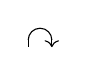
\begin{tikzpicture}[scale=0.03em]
    \draw (0,0) arc (0:180:0.5);
    \draw (0,0) edge[->] (0,-0.3);
    \draw (-1,0) edge (-1,-0.3);
  \end{tikzpicture}
}
\newcommand\arcfromtop{
  
\begin{tikzpicture}[scale=0.03em]
    \draw (0,0) arc (180:360:0.5);
    \draw (0,0) edge[->] (0,0.3);
    \draw (1,0) edge (1,0.3);
  \end{tikzpicture}
}

\newcommand{\Elim}{\mathsf{Elim}}
\newcommand{\elim}{\mathsf{elim}}
\newcommand{\Rec}{\mathsf{Rec}}
\newcommand{\record}{\mathsf{record}}
\newcommand{\funext}{\mathsf{funext}} \newcommand{\Q}{\mathsf{Q}}
\renewcommand{\T}{\mathsf{T}} \newcommand{\leaf}{\mathsf{leaf}}
\newcommand{\node}{\mathsf{node}} \newcommand{\perm}{\mathsf{perm}}
\newcommand{\coe}{\mathsf{coe}} \newcommand{\vz}{\mathsf{vz}}
\newcommand{\vs}{\mathsf{vs}} \newcommand{\untr}{\mathsf{untr}}
\newcommand{\from}{\mathsf{from}}
\newcommand{\fromeq}{{\mathsf{from}\hspace{-0.3em}\equiv}}
\newcommand{\fromsimeq}{{\mathsf{from}\hspace{-0.3em}\simeq}}
\newcommand{\Model}{\mathsf{Model}}
\newcommand{\DModel}{\mathsf{DModel}}
\newcommand{\module}{\mathsf{module}}
\newcommand{\open}{\mathsf{open}}
\renewcommand{\P}{\mathsf{P}} \newcommand{\Bool}{\mathsf{Bool}}
\newcommand{\true}{\mathsf{true}} \newcommand{\false}{\mathsf{false}}
\renewcommand{\not}{\mathsf{not}} \newcommand{\0}{\mathsf{0}}
\newcommand{\1}{\mathsf{1}} \renewcommand{\Pr}{\mathsf{Pr}}
\newcommand{\PrNat}{\mathsf{PrNat}} \newcommand{\J}{\mathsf{J}}
\newcommand{\wkV}{\mathsf{wkV}} \renewcommand{\r}[1]{{\P_{#1}}}
\newcommand{\stab}{\mathsf{stab}} \newcommand{\NTy}{\mathsf{NTy}}
\newcommand{\isDec}{\mathsf{isDec}} \newcommand{\dec}{\mathsf{dec}}
\newcommand{\yes}{\mathsf{yes}} \newcommand{\no}{\mathsf{no}}
\newcommand{\case}{\mathsf{case}} \newcommand{\inj}{\mathsf{inj}}
\newcommand{\K}{\mathsf{K}} \newcommand{\lb}{\langle}
\newcommand{\rb}{\rangle} \newcommand{\Decl}{\mathsf{Decl}}
\newcommand{\Core}{\mathsf{Core}} \newcommand{\IND}{\mathsf{ind}}
\newcommand{\Id}{\mathsf{Id}} \newcommand{\Base}{\mathsf{Base}}
\newcommand{\Setoid}{\mathsf{Setoid}}
\newcommand{\FamSetoid}{\mathsf{FamSetoid}}
\newcommand{\prop}{\mathsf{prop}} \newcommand{\resp}{\mathsf{resp}}
\newcommand{\transport}{\mathsf{transport}}
\newcommand{\I}{\mathsf{I}} \newcommand{\E}{\mathsf{E}}
\newcommand{\transp}{\mathsf{transp}}
\newcommand{\Transp}{\mathsf{Transp}}
\newcommand{\W}{\mathsf{W}}
\newcommand{\Fin}{\mathsf{Fin}} \newcommand{\fzero}{\mathsf{fzero}}
\newcommand{\fsuc}{\mathsf{fsuc}}
\newcommand{\inv}{\mathsf{inv}}
\newcommand{\con}{\mathsf{con}}
\newcommand{\LEFT}{\mathsf{left}}
\newcommand{\RIGHT}{\mathsf{right}}
\newcommand{\seg}{\mathsf{seg}}
\newcommand{\Int}{\mathsf{Int}}
\renewcommand{\in}{\mathbin{\hat:}}
%% \renewcommand{\hat}[1]{{\color{BrickRed}{#1}}}
\newcommand{\vdashh}{\mathbin{\hat\vdash}}
\newcommand{\rah}{\mathbin{\hat\ra}}
\newcommand{\commah}{\hat,\,}
\newcommand{\timesh}{\mathbin{\hat\times}}
\newcommand{\eqh}{\mathbin{\hat=}}
\newcommand{\TR}{\hat{\mathsf{tr}}}
\newcommand{\ap}{\hat{\mathsf{ap}}}
\newcommand{\apd}{\hat{\mathsf{apd}}}
\renewcommand{\tt}{\hat{\mathsf{tt}}}
\newcommand{\Tel}{\hat{\mathsf{Tel}}}
\newcommand{\Type}{\hat{\mathsf{Type}}}
\newcommand{\emptytel}{\hat{\epsilon}}
\newcommand{\telext}{\mathbin{\hat{\lhd}}}
\newcommand{\ltel}{\hat{\ll}}
\newcommand{\rtel}{\hat{\rr}}
\newcommand\pp{\ensuremath{\hat{\mathbin{+\mkern-10mu+}}}}
%% \newcommand{\semicol}{\hat;\,}
%% \newcommand{\targetass}{\hat{\Gamma}\semicol}
%\newcommand{\targetass}{;}

\newcommand{\type}{\mathsf{type}}
\newcommand{\Cl}{\mathsf{Cl}}
\newcommand{\pack}{\mathsf{pack}}

\title{Closure Conversion for Dependent Type Theory}
\subtitle{With Type-Passing Polymorphism\thanks{This work was supported by the European Union, co-financed by the European
Social Fund (EFOP-3.6.3-VEKOP-16-2017-00002).}}
\author{András Kovács}
\institute{Eötvös Loránd University, Budapest}
\date{TYPES 2018, 20 June 2018}


\begin{document}

\frame{\titlepage}


\begin{frame}{Advertising}


William J. Bowman and Amal Ahmed: \emph{Typed Closure Conversion for the Calculus of Constructions}, PLDI 2018, Philadelphia.

\begin{itemize}
\item
Significant overlap with the current talk. I was unaware of the
preprint until a kind TYPES reviewer pointed it out to me.
\item
The basic technical idea (abstract closures) is the same as here (independent validation!).
\item
I encourage interested people to read this paper for details.
\end{itemize}

\end{frame}

\begin{frame}{Motivation}
  \begin{itemize}
  \item
    Variants of dependent type theory proliferate: quantitative, cubical, guarded, etc.
  \item
    We would like to add: \emph{type theory with precise memory layout control.}
  \item
    Hopefully eventually complementing the resource usage control of quantitative
    type theories.
  \item Benefits:
    \begin{itemize}
    \item As front-end language: more control for programmers
      %% Talk about examples
    \item As intermediate language: precisely typed, memory-safe transformations,
          single language for a large universe of runtime objects.
    \end{itemize}
  \end{itemize}
\end{frame}

\begin{frame}{Ingredients of memory layout control}

  We need to make some new distinctions:

  \begin{itemize}
  \item Types vs. runtime type codes
  \item Closed functions vs. closures
  \item Consecutive layout vs. pointers
  \item Storage location
  \item Alignment
  \item (more things)
  \end{itemize}
(Also: should we allow internal abstraction over these distinctions?)
\end{frame}

\begin{frame}{Ingredients of memory layout control}

  We need to make some new distinctions:

  \begin{itemize}
  \item {\color{red} Types vs. runtime type codes}
  \item {\color{red} Closed functions vs. closures}
  \item Consecutive layout vs. pointers
  \item Storage location
  \item Alignment
  \item (more things)
  \end{itemize}
(Also: should we allow internal abstraction over these distinctions?)
\end{frame}

\begin{frame}{Current contribution}

  A small type theory where:
  \begin{itemize}
  \item There aren't general dependent functions, only closed functions and closures.
  \item But general dependent functions remain admissible, through closure conversion.
  \item Type codes use closures to represent type dependency.
  \end{itemize}
\end{frame}


\begin{frame}{Type-passing polymorphism}

  Closures in type codes allow efficient memory layout computation at runtime.\\~\\
  For example: computing the size of a value with $\Sigma$-type. \\~\\
  See: \emph{Harper \& Morrisett: Compiling Polymorphism Using Intensional Type Analysis}. \\~\\
  Intensional (synonymously: type-passing) polymorphism generalizes type erasure (e. g. GHC Haskell) and monomorphization (e. g. Rust, C++).e
  We don't want to \emph{rule out} type-passing polymorphism down the compilation pipeline.

\end{frame}

\begin{frame}{The type theory (1)}

Judgements:
\begin{gather*}
  \Gamma \vdash  \hspace{2em}  \Gamma \vdash A\,\type_i \hspace{2em} \Gamma \vdash t : A
\end{gather*}
Universes:
\begin{gather*}
  \infer{\Gamma \vdash \U_i\,\,\type_{i+1}}{}
  \hspace{2em}
  \infer{\Gamma \vdash \El\,A : \type_i}{\Gamma \vdash A : \U_i}
\end{gather*}
Closed functions:
\begin{gather*}
  \infer{\Gamma \vdash (a : A)\ra B\,\,\type_{\max(i,\,j)}}{\Gamma \vdash A\,\type_i & \Gamma, a : A \vdash B\,\type_j}
  \hspace{1em}
  \infer{\Gamma \vdash \lambda a.\,t : (a : A)\ra B}{\boldsymbol{\cdot},\,a : A \vdash t : B}
\end{gather*}
\begin{itemize}
\item Standard application, $\beta$ and $\eta$ for closed functions.
\item Standard $\Sigma$ types and $\top$ (unit type).
\end{itemize}
\end{frame}

\begin{frame}{}

  Closed functions are quite restricted.\\~\\
  The usual polymorphic identity function isn't possible: $\lambda A.\,\lambda (x : {\color{red}A}).\, x$.\\~\\
  Instead, we may have $\lambda(A,\,x).\,x : (x : \Sigma(A : U).\,\El\,A) \ra \El\,(\pi_1\,x)$\\~\\
  Also: a function with type $A \ra B \ra C$ can never return its first argument.

\end{frame}

\begin{frame}{Closures}

\begin{gather*}
  \infer{\Gamma \vdash \Cl\,(a : A)\,B\,\,\type_{\max(i,\,j)}}{\Gamma \vdash A\,\type_i & \Gamma, a : A \vdash B\,\type_j}
\end{gather*}
\begin{gather*}
\infer{\Gamma \vdash \pack\,E\,env\,\,t : \Cl\,(a : A[e\mapsto env])\,(B[ea \mapsto (env,\,a)])}{\boldsymbol{\cdot} \vdash E : \U_i & \Gamma \vdash env : \El\, E & \boldsymbol{\cdot} \vdash t : (ea : \Sigma(e : \El\,E).A) \ra B}
\end{gather*}
\begin{gather*}
  \infer{\Gamma \vdash t\,u : B[a \mapsto u]}{\Gamma \vdash t : \Cl\,(a : A)\,B & \Gamma \vdash u : A}
\end{gather*}
\begin{gather*}
  \infer{\Gamma \vdash t \equiv u}{\Gamma \vdash t : \Cl\,(a : A)\,B & \Gamma \vdash u : \Cl\,(a : A)\,B & \Gamma,\,a : A \vdash t\,a \equiv u\,a}
\end{gather*}
\begin{gather*}
  (\pack\,E\,env\,\,t)\,u \equiv t\,(env,\,u)
\end{gather*}
\end{frame}

\begin{frame}{Type codes}

Universe:

\begin{gather*}
\infer{\Gamma \vdash \U'_i : \U_{i+1}}{}\hspace{2em} \El\,\U'_i\equiv \U_i
\end{gather*}

Codes for $Cl$:

\begin{gather*}
  \infer{\Gamma \vdash \mathsf{Cl'}\,A\,B : \U_{\max(i,\,j)}}
        {\Gamma \vdash A : \U_i & \Gamma \vdash B : \Cl\,(\El\,A)\,(\U_j)}
  \hspace{2.5em}
  \El\,(\mathsf{Cl'}\,A\,B)\equiv \Cl\,(a : \El\,A)\,(\El\,(B\,a))
\end{gather*}
\\~\\
Analogously for $\Sigma$ and closed functions. Dependency is represented by $\Cl$.

\end{frame}

\begin{frame}
\\~\\
\\~\\
Polymorphic identity function with closures:
  \begin{alignat*}{5}
    & \mathsf{id} : \Cl(A : \U)(\Cl(x : \El\,A)(\El\,A)) \\
    & \mathsf{id} :\equiv \pack\,\top'\,\tt\,(\lambda(\_,\,A).\, \pack\,\U'\,A\,(\lambda(A,\,x).\,x))
\end{alignat*}
\end{frame}

\begin{frame}{Closure conversion}

General function abstraction (called $\lambda{x}.t$) is admissible.

\end{document}
